\documentclass[border=10pt]{standalone}

\usepackage{tikz}
\usepackage{tikzsymbols}
\usetikzlibrary{calc,patterns,shapes.geometric}

\def\centerarc[#1](#2)(#3:#4:#5){\draw[#1] ($(#2)+({#5*cos(#3)},{#5*sin(#3)})$) arc (#3:#4:#5);}

\begin{document}
	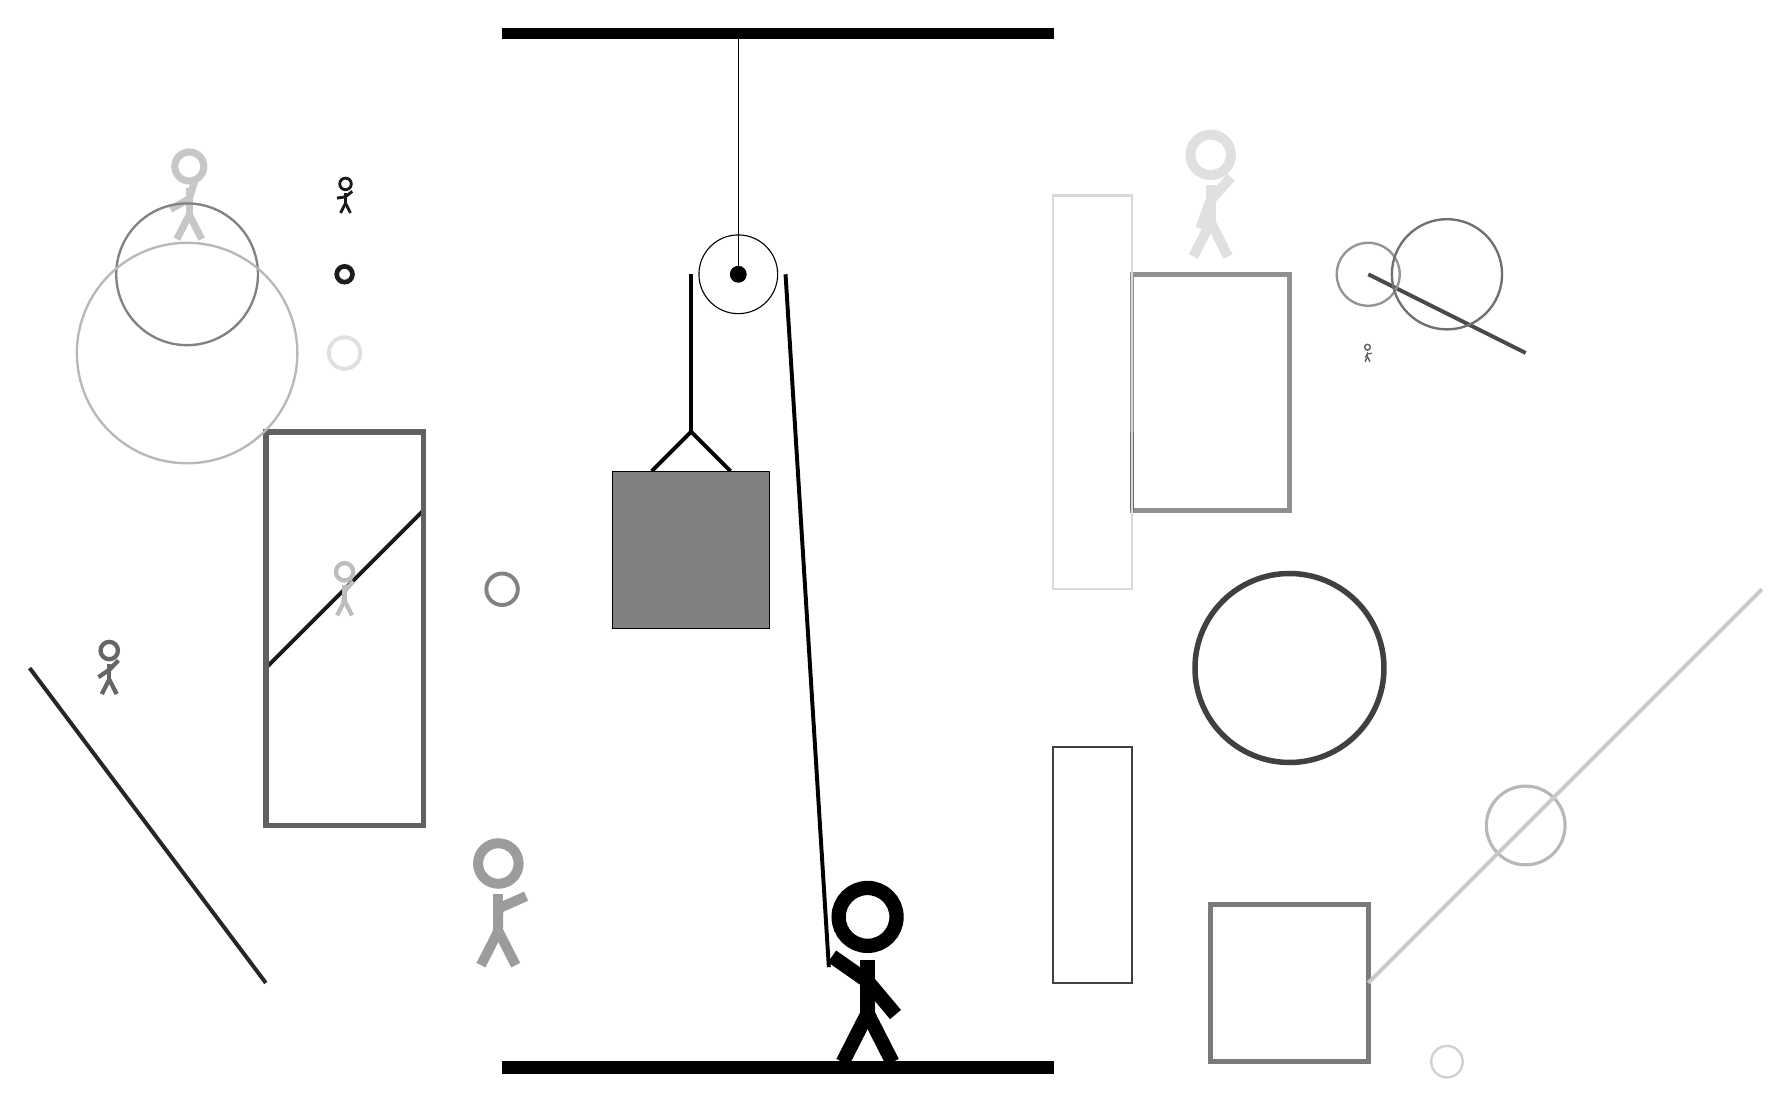
\begin{tikzpicture}
		%%%%% START %%%%%
		
		\draw[fill=black] (-2, 10) rectangle (5, 10.125);
		
		\draw (1, 7) circle (0.5);
		\draw[fill=black] (1, 7) circle (0.1);
		\draw (1, 10) -- (1, 7);
		
		\node[line width=0.7mm, color=black!39] at (-2, -1) {\Strichmaxerl[7][89][24]};
		
		\node[line width=0.2mm, color=black!62] at (9, 6) {\Strichmaxerl[1][63][3]};
		\draw[line width=0.6mm, color=black!44] (6, 4) rectangle (8, 7);
		\node[line width=0.3mm, color=black!22] at (-6, 8) {\Strichmaxerl[5][30][73]};
		
		\draw [line width=0.5mm, color=black!49](-2, 3) circle (0.2);
		\draw [line width=0.3mm, color=black!18](10, -3) circle (0.2);
		\node[line width=0.2mm, color=black!90] at (-4, 8) {\Strichmaxerl[2][9][39]};
		\draw[line width=0.5mm, color=black!71](9, 7) -- (11, 6);
		\node[line width=0.2mm, color=black!60] at (-7, 2) {\Strichmaxerl[3][34][46]};
		\draw[line width=0.5mm, color=black!90](-3, 4) -- (-5, 2);
		
		\draw[line width=0.6mm, color=black!52] (7, -1) rectangle (9, -3);
		\draw [line width=0.6mm, color=black!89](-4, 7) circle (0.1);
		\node[line width=0.4mm, color=black!12] at (7, 8) {\Strichmaxerl[7][70][48]};
		\draw [line width=0.5mm, color=black!12](-4, 6) circle (0.2);
		\draw [line width=0.3mm, color=black!49](-6, 7) circle (0.9);
		\draw [line width=0.3mm, color=black!42](9, 7) circle (0.4);
		\draw [line width=0.7mm, color=black!75](8, 2) circle (1.2);
		
		\draw[line width=0.6mm, color=black!58] (6, 4) rectangle (6, 5);
		\draw[line width=0.3mm, color=black!75] (5, 1) rectangle (6, -2);
		\draw[line width=0.7mm, color=black!62] (-3, 0) rectangle (-5, 5);
		\draw[line width=0.5mm, color=black!85](-5, -2) -- (-8, 2);
		\node[line width=0.5mm, color=black!26] at (-4, 3) {\Strichmaxerl[3][84][48]};
		\draw [line width=0.3mm, color=black!56](10, 7) circle (0.7);
		\draw[line width=0.3mm, color=black!15] (5, 3) rectangle (6, 8);
		\draw [line width=0.3mm, color=black!28](-6, 6) circle (1.4);
		
		\draw [line width=0.4mm, color=black!28](11, 0) circle (0.5);
		\draw[line width=0.5mm, color=black!21](9, -2) -- (14, 3);
		
		\draw[line width=0.5mm] (-0.1, 4.5) -- (0.4, 5.0) -- (0.9, 4.5);
		\draw[fill=black!50] (-0.6, 4.5) rectangle (1.4, 2.5);
		
		\draw[line width=0.5mm] (0.4, 7) -- (0.4, 5.0);
		\centerarc[line width=0.5mm](1, 7)(0:180:0.6);
		\draw[line width=0.5mm](1.6, 7) -- (2.15, -1.8);
		
		\node at (2.6, -1.9) {\Strichmaxerl[10][-35][-50]};
		
		\draw[fill=black] (-2, -3) rectangle (5, -3.15);
		
		%%%%% END %%%%%
	\end{tikzpicture}
\end{document}